% Don't touch this %%%%%%%%%%%%%%%%%%%%%%%%%%%%%%%%%%%%%%%%%%%
\documentclass[12pt]{article}
\usepackage{fullpage}
\usepackage[left=1in,top=1in,right=1in,bottom=1in,headheight=3ex,headsep=3ex]{geometry}
\usepackage{graphicx}
\usepackage{float}
\usepackage{array}


\newcommand{\blankline}{\quad\pagebreak[2]}
%%%%%%%%%%%%%%%%%%%%%%%%%%%%%%%%%%%%%%%%%%%%%%%%%%%%%%%%%%%%%%

% Modify Course title, instructor name, semester here %%%%%%%%

\title{Review}
\author{PHY250 - Fall 2021}
\date{}

%%%%%%%%%%%%%%%%%%%%%%%%%%%%%%%%%%%%%%%%%%%%%%%%%%%%%%%%%%%%%%

% Don't touch this %%%%%%%%%%%%%%%%%%%%%%%%%%%%%%%%%%%%%%%%%%%
\usepackage[sc]{mathpazo}
%\linespread{1.05} % Palatino needs more leading (space between lines)
\usepackage[T1]{fontenc}
\usepackage[mmddyyyy]{datetime}% http://ctan.org/pkg/datetime
\usepackage{advdate}% http://ctan.org/pkg/advdate
\newdateformat{syldate}{\twodigit{\THEMONTH}/\twodigit{\THEDAY}}
\newsavebox{\MONDAY}\savebox{\MONDAY}{Mon}% Mon
\newcommand{\week}[1]{%
%  \cleardate{mydate}% Clear date
% \newdate{mydate}{\the\day}{\the\month}{\the\year}% Store date
  \paragraph*{\kern-2ex\quad #1, \syldate{\today} - \AdvanceDate[4]\syldate{\today}:}% Set heading  \quad #1
%  \setbox1=\hbox{\shortdayofweekname{\getdateday{mydate}}{\getdatemonth{mydate}}{\getdateyear{mydate}}}%
  \ifdim\wd1=\wd\MONDAY
    \AdvanceDate[7]
  \else
    \AdvanceDate[7]
  \fi%
}
%\usepackage{setspace}
\usepackage{multicol}
%\usepackage{indentfirst}
\usepackage{fancyhdr,lastpage}
\usepackage{url}
\pagestyle{fancy}
\usepackage{hyperref}
\usepackage{lastpage}
\usepackage{amsmath}
\usepackage{layout}

\lhead{}
\chead{}
%%%%%%%%%%%%%%%%%%%%%%%%%%%%%%%%%%%%%%%%%%%%%%%%%%%%%%%%%%%%%%

% Modify header here %%%%%%%%%%%%%%%%%%%%%%%%%%%%%%%%%%%%%%%%%
%\rhead{\footnotesize Text in header}

%%%%%%%%%%%%%%%%%%%%%%%%%%%%%%%%%%%%%%%%%%%%%%%%%%%%%%%%%%%%%%
% Don't touch this %%%%%%%%%%%%%%%%%%%%%%%%%%%%%%%%%%%%%%%%%%%
\lfoot{}
\cfoot{\small \thepage/\pageref*{LastPage}}
\rfoot{}

\usepackage{array, xcolor}
\usepackage{color,hyperref}
\definecolor{clemsonorange}{HTML}{EA6A20}
\hypersetup{colorlinks,breaklinks,linkcolor=clemsonorange,urlcolor=clemsonorange,anchorcolor=clemsonorange,citecolor=black}

\begin{document}

\maketitle




% First Section %%%%%%%%%%%%%%%%%%%%%%%%%%%%%%%%%%%%%%%%%%%%


\newcounter{example}
\setcounter{example}{1}

\section*{Exercise \theexample}
Water flows steadily from an open tank. The elevation of point 1 is $H$, and the elevation
of points 2 and 3 is $h$. The cross-sectional area at point 2 is $A_2$
at point 3 it is $A_3$. The area of the tank is very
large compared with the cross-sectional area of the pipe. Assuming
that Bernoulli’s equation applies, compute (a) the discharge
rate  and (b) the gauge pressure at point 2.

\vspace{5mm}

\begin{figure}[h!]
    \begin{center}
      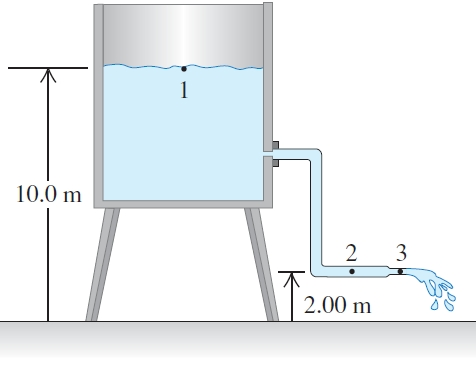
\includegraphics[height=2.5in]{images/1.jpg}
      \caption{Exercise \theexample }
      \label{1}
    \end{center}
  \end{figure}

% First Section %%%%%%%%%%%%%%%%%%%%%%%%%%%%%%%%%%%%%%%%%%%%
\stepcounter{example}

\section*{Exercise \theexample}

A slender, uniform,
metal rod with mass M
is pivoted without friction about
an axis through its midpoint and
perpendicular to the rod. A horizontal
spring with force constant
k is attached to the lower end of
the rod, with the other end of the
spring attached to a rigid support.
If the rod is displaced by a
small angle from the vertical
 and released, show
that it moves in angular SHM
and calculate the period. 


% \vspace{5mm}

\begin{figure}[h!]
    \begin{center}
      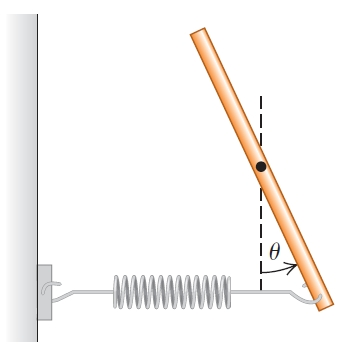
\includegraphics[height=2.5in]{images/3.jpg}
      \caption{Exercise \theexample }
      \label{3}
    \end{center}
  \end{figure}


% First Section %%%%%%%%%%%%%%%%%%%%%%%%%%%%%%%%%%%%%%%%%%%%
\stepcounter{example}

\section*{Exercise \theexample}

A vibrating string 50.0 cm long is under a tension of
1.00 N. The results from five successive stroboscopic pictures are
shown in Fig. \ref{4}. The strobe rate is set at 5000 flashes per
minute, and observations reveal that the maximum displacement
occurred at flashes 1 and 5 with no other maxima in between. (a)
Find the period, frequency, and wavelength for the traveling waves
on this string. (b) In what normal mode (harmonic) is the string
vibrating? (c) What is the speed of the traveling waves on the
string? (d) How fast is point P moving when the string is in (i)
position 1 and (ii) position 3? (e) What is the mass of this string?



\begin{figure}[h!]
    \begin{center}
      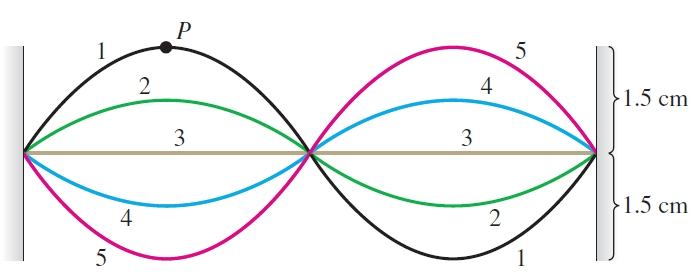
\includegraphics[height=2.3in]{images/4.jpg}
      \caption{Exercise \theexample }
      \label{4}
    \end{center}
  \end{figure}


%   Two identical thin
% rods, each with mass m and
% length L, are joined at right
% angles to form an L-shaped
% object. This object is balanced
% on top of a sharp edge. If the L-shaped object
% is deflected slightly, it oscillates.
% Find the frequency of oscillation.

% \vspace{5mm}

% \begin{figure}[h!]
%     \begin{center}
%       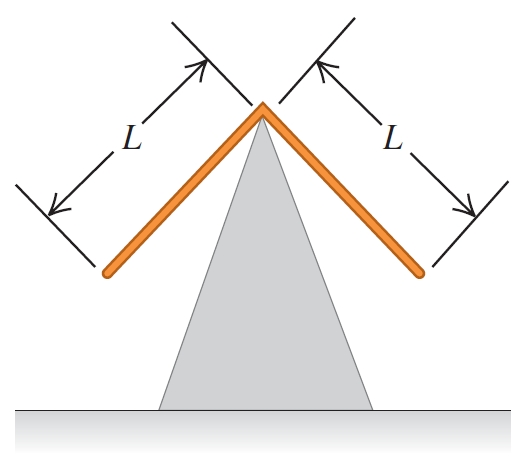
\includegraphics[height=2.5in]{images/2.jpg}
%       \caption{Exercise \theexample }
%       \label{2}
%     \end{center}
%   \end{figure}



\end{document}


